\section{Question 3}
The fourth cache model doesn't make any sense. The different cache models in
this lab are motivated by the desire of parallelizing cache access and address
translation.

If the cache is physically index, it means the cache access cannot start unil
after address translation. Since we waited for address translation anyway, we
might as well use the physical address for the tag. There's no reason to deal
with the additional complexities of using virtual tagging.

\section{Question 4}
Having more than one process at a time means that each process will have its
own page tables, and therefore the virtual-to-physical mapping can change
during cache operation.

The physically-indexed physically-tagged cache isn't impacted by this change at
all, since it's oblivious to address translation.

The virtually-indexed virtually-tagged cache 

The virtually-indexed physically-tagged cache is equipped to deal with this
change. If the mapping changes, the tag will not match, so the cache will not
give a bad answer by mistake. The cache's design has to deal with aliasing
(different virtual addresses pointing to the same physical address) for the
single-process case, so multiple processes don't introduce a change.

The TAs would have to modify the address translation routine in our source code
to simulate different processes, so I doubt that will be part of the tests. 

\section{Question 5}

I stripped the supplied \texttt{caches} pintool into a pintool that counts the
read and write memory accesses, as well as the aligned reads and writes. The
summaries are presented in figure \ref{q5:unaligned_accesses}.

\begin{figure}[htb]
\center
\begin{tabular}{lrrr}
\hline
Test & \% unaligned reads & \% unaligned writes & \% unaligned accesses \\
\hline
applu & 0.00019\% & 0.00047\% & 0.00023\%  \\
\hline
art & 0.00013\% & 0.00050\% & 0.00019\%  \\
\hline
bzip2 & 0.24491\% & 0.36827\% & 0.28971\%  \\
\hline
cc1 & 0.04994\% & 0.01413\% & 0.03852\%  \\
\hline
crafty & 0.02442\% & 0.01042\% & 0.01913\%  \\
\hline
equake & 0.01114\% & 0.01851\% & 0.01239\%  \\
\hline
gap & 0.08745\% & 0.04416\% & 0.07358\%  \\
\hline
gzip & 0.14022\% & 0.12515\% & 0.13500\%  \\
\hline
mesa & 0.07836\% & 0.08633\% & 0.08100\%  \\
\hline
parser & 0.07013\% & 0.00846\% & 0.04782\%  \\
\hline
swim & 0.00003\% & 0.00007\% & 0.00004\%  \\
\hline
{}Averages & 0.06426\% & 0.06150\% & 0.06342\%  \\
\hline
\end{tabular}

\caption{The percentage of unaligned memory accesses out of the total memory
accesses for the SPEC 2000 benchmark suite. }
\label{q5:unaligned_accesses}
\end{figure}

The bulk of unaligned accesses come from \texttt{bzip2}, which is a
compression tool, and therefore it works with streams of bytes. Other
significant sources of unaligned accesses are also processing streams
of bytes -- \textt{cc} compiles C code, and \textt{parser} presumably builds an
AST out of some language. The one that didn't come to my mind waas
\texttt{mesa}, which is a software OpenGL implementation, and therefore has to
work with a software framebuffer.

The assumption of aligned accesses seems to make sense. The numbers reported
above are an upper bound of unaligned accesses because, from a cache
perspective, byte accesses can be satisfied even if they're unaligned, and
multibyte accesses are only problematic if they span across 2 cache blocks.
Furthermore, the applications which are most impacted by unaligned access don't
really run on consumer computers -- most people don't compile their code, and a
vast majority of desktop and mobile platforms have accelerated graphics
nowadays.


\section{X 1}
Figure \ref{q1:frequencies} shows the dependencies obtained as suggested in the
lab handout.

\begin{figure}[htb]
  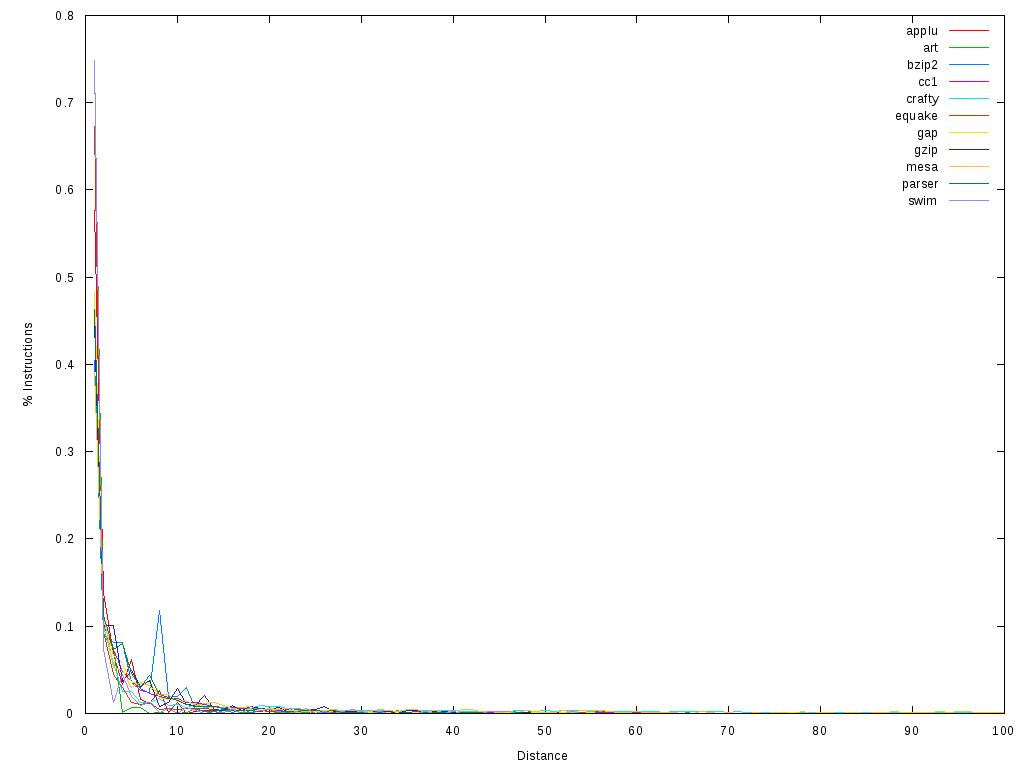
\includegraphics[width=6.8in]{6.823/lab1/figs/frequencies.png}
  \caption{Instruction dependency frequencies for the 11 benchmarks. }
  \label{q1:frequencies}.
\end{figure}

The graph is not too helpful, except to tell us that most instructions depend
on registers written in the past 4-5 instructions. Therefore, we use figure
\ref{q1:frequencies_zoom} to take a better look at the dependencies at most 5
instructions apart.

\begin{figure}[htb]
  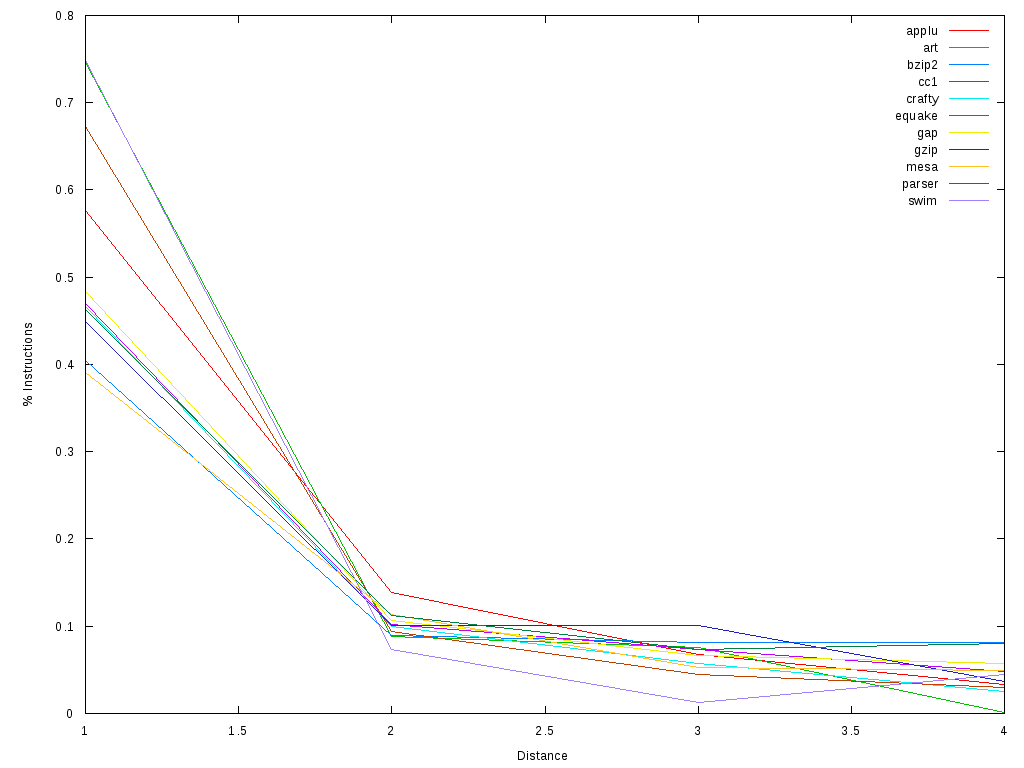
\includegraphics[width=6.8in]{6.823/lab1/figs/frequencies_zoom.png}
  \caption{Instruction dependency frequencies for the 11 benchmarks. }
  \label{q1:frequencies_zoom}.
\end{figure}

Given the dependency statistics, it seesms like architecture A would be
significantly faster than architecture B. In each benchmark, between 40\% -
80\% of the instructions depend on the previous instruction. In architecture B,
all instructions with dependencies on the previous instruction would have to be
stalled for 1 cycle, while the previous instruction writes its registers. This
means 40\%-80\% pipeline bubbles, which could be avoided by the forwarding
circuitry.

\section{X 2}

Figure \ref{q2:reg_frequencies} shows the per-register breakdown for the
instruction dependency. For each register and instruction distance, we computed
the proportion of dependencies that are owed to that register. We averaged the
values for each benchmark. We only plotted registers which contributed a
dependency of at least 0.005\% on for at least one distance.

\begin{figure}[htb]
  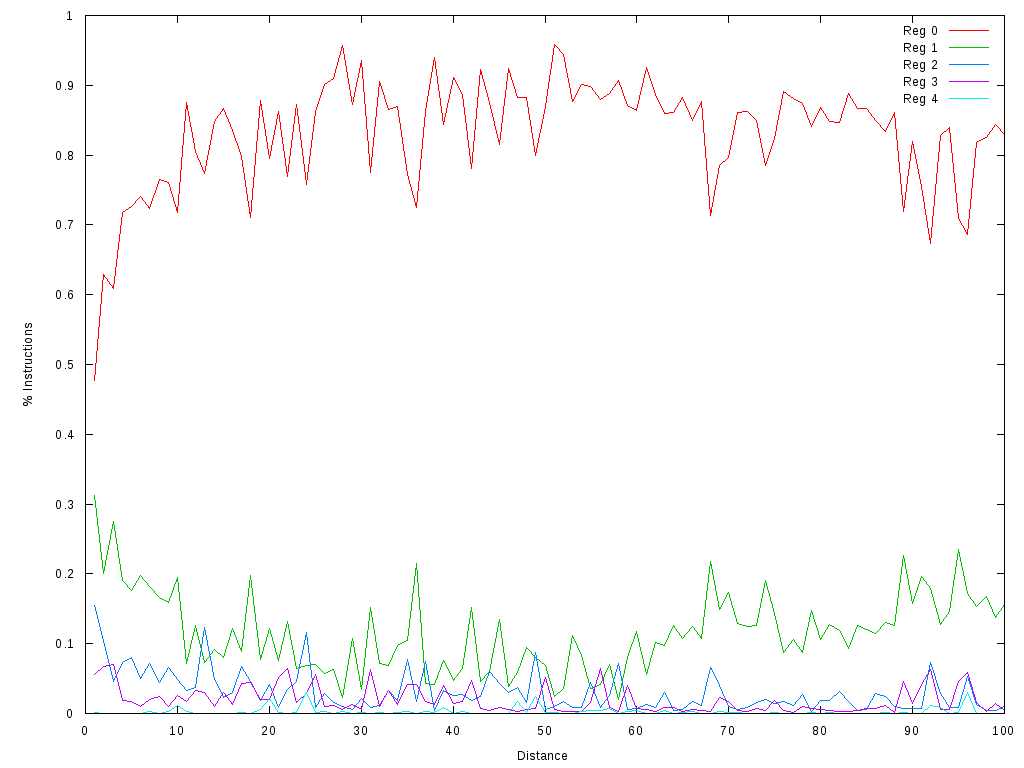
\includegraphics[width=6.8in]{6.823/lab1/figs/reg_frequencies.png}
  \caption{Instruction dependency frequencies broken down by register. }
  \label{q2:reg_frequencies}.
\end{figure}

The graph suggests that a few registers are responsible for most dependencies.
This is not very surprising, given the x86 architecture's predilection to use
the \texttt{eax} register as an accumulator, \texttt{esi} and \texttt{edi}
as pointers, and the presence of a condition flags register.

The best (but most difficult to implement) suggestion would be to give the
instruction set a makeover so it looks more like a RISC instruction set. It's
not cool to have 8 registers, and instructions with limitations on the registers
they can use. However, as Alpha found out, this strategy might not work
commercially.\footnote{One could argue that, even though the strategy failed in
the 1990s, we're living in a different landscape right now, where many servers
are running some flavor of UNIX/Linux. So, maybe the instruction set will be
redesigned one day.}

Assuming we're stuck with the ISA, it seems that (limited) forwarding is very
worth-while. The dependencies seem to taper off after 4 cycles, so it's
probably not worth forwarding for more than 4 cycles. This is important in
super-pipelined architectures, like the latest Pentiums and Core processors.
